\documentclass{beamer}
\mode<presentation>
\usepackage{amsmath}
\usepackage{amssymb}
%\usepackage{advdate}
\usepackage{adjustbox}
\usepackage{subcaption}
\usepackage{enumitem}
\usepackage{multicol}
\usepackage{mathtools}
\usepackage{listings}
\usepackage{physics}
\usepackage{url}
\def\UrlBreaks{\do\/\do-}
\usetheme{Boadilla}
\usecolortheme{lily}
\setbeamertemplate{footline}
{
  \leavevmode%
  \hbox{%
  \begin{beamercolorbox}[wd=\paperwidth,ht=2.25ex,dp=1ex,right]{author in head/foot}%
    \insertframenumber{} / \inserttotalframenumber\hspace*{2ex} 
  \end{beamercolorbox}}%
  \vskip0pt%
}

\providecommand{\nCr}[2]{\,^{#1}C_{#2}} % nCr
\providecommand{\nPr}[2]{\,^{#1}P_{#2}} % nPr
\providecommand{\mbf}{\mathbf}
\providecommand{\pr}[1]{\ensuremath{\Pr\left(#1\right)}}
\providecommand{\qfunc}[1]{\ensuremath{Q\left(#1\right)}}
\providecommand{\sbrak}[1]{\ensuremath{{}\left[#1\right]}}
\providecommand{\lsbrak}[1]{\ensuremath{{}\left[#1\right.}}
\providecommand{\rsbrak}[1]{\ensuremath{{}\left.#1\right]}}
\providecommand{\brak}[1]{\ensuremath{\left(#1\right)}}
\providecommand{\lbrak}[1]{\ensuremath{\left(#1\right.}}
\providecommand{\rbrak}[1]{\ensuremath{\left.#1\right)}}
\providecommand{\cbrak}[1]{\ensuremath{\left\{#1\right\}}}
\providecommand{\lcbrak}[1]{\ensuremath{\left\{#1\right.}}
\providecommand{\rcbrak}[1]{\ensuremath{\left.#1\right\}}}
\theoremstyle{remark}
\newtheorem{rem}{Remark}
\newcommand{\sgn}{\mathop{\mathrm{sgn}}}
\providecommand{\abs}[1]{\left\vert#1\right\vert}
\providecommand{\res}[1]{\Res\displaylimits_{#1}} 
\providecommand{\norm}[1]{\lVert#1\rVert}
\providecommand{\mtx}[1]{\mathbf{#1}}
\providecommand{\mean}[1]{E\left[ #1 \right]}
\providecommand{\fourier}{\overset{\mathcal{F}}{ \rightleftharpoons}}
%\providecommand{\hilbert}{\overset{\mathcal{H}}{ \rightleftharpoons}}
\providecommand{\system}{\overset{\mathcal{H}}{ \longleftrightarrow}}
	%\newcommand{\solution}[2]{\textbf{Solution:}{#1}}
%\newcommand{\solution}{\noindent \textbf{Solution: }}
\providecommand{\dec}[2]{\ensuremath{\overset{#1}{\underset{#2}{\gtrless}}}}
\newcommand{\myvec}[1]{\ensuremath{\begin{pmatrix}#1\end{pmatrix}}}
\let\vec\mathbf

\lstset{
%language=C,
frame=single, 
breaklines=true,
columns=fullflexible
}

\numberwithin{equation}{section}

\lstset{
  language=Python,
  basicstyle=\ttfamily\small,
  keywordstyle=\color{blue},
  stringstyle=\color{orange},
  numbers=left,
  numberstyle=\tiny\color{gray},
  breaklines=true,
  showstringspaces=false
}

\title{Problem 2.7.30}
\author{EE25BTECH11018- Darisy Sreetej}

\date{\today} 
\begin{document}

\begin{frame}
\titlepage
\end{frame}

\begin{frame}
\frametitle{Problem Statement}
%
 Find the value of $k$ so that the area of $\triangle$$ABC$ with $\vec{A}\brak{k+1,1}$ , $\vec{B}\brak{4,-3}$ and $\vec{C}\brak{7, -k}$ is $6$ square units
\end{frame}
%\subsection{Literature}

\begin{frame}
\frametitle{Formula}
\setcounter{section}{1}
%\framesubtitle{Literature}
\begin{align}
\text{Area\brak{\triangle ABC}}&=\frac12\norm{\brak{\vec{B}-\vec{A}}\times\brak{\vec{C}-\vec{A}}}
\end{align}
\end{frame}
\begin{frame}
\frametitle{Solution}

Here according to problem , the Area of $\triangle$$ABC$ is $6$ square units\\
Therefore,
\begin{align}
\frac{1}{2}\norm{\brak{\vec{B}-\vec{A}}\times\brak{\vec{C}-\vec{A}}}=6\\
\frac{1}{2}\norm{\myvec{4\\-3} - \myvec{k+1\\1} \times \myvec{7\\-k} - \myvec{k+1\\1}}=6\\
\frac{1}{2}\norm{\myvec{3-k\\-4}\times\myvec{6-k\\-k-1}}=6
\end{align}
\begin{align}
\mdet{\brak{3-k}\brak{-k-1} - \brak{-4}\brak{6-k}}=12 \\
\mdet{k^2-6k+21}=12
\end{align}

\end{frame}
\begin{frame}
\frametitle{Solution}
Case 1 :
\begin{align}
   k^2-6k+24=12\\
k^2-6k+9=0\\
(k-3)^2=0\\
k=3
\end{align}
Case 2 :
\begin{align}
k^2-6k+24=-12\\
k^2-6k+33=0\\
\end{align}
Discriminant: $D=-96$.\\ Since the discriminant is negative , there is no real solution for this case.\\

Thus , k=3
\end{frame}
\subsection{Plot}
\begin{frame}[fragile]
\frametitle{Plot}

\begin{figure}[h!]
   \centering
   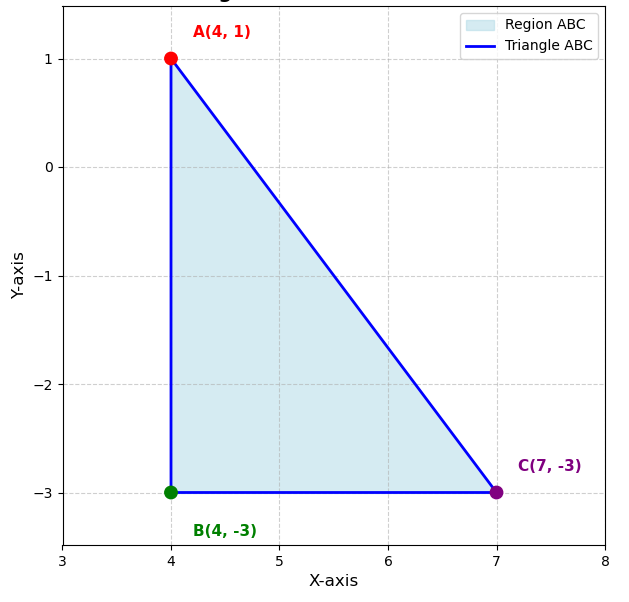
\includegraphics[width=0.7\columnwidth]{figs/fig.png}
	\caption{}
   \label{stemplot}
\end{figure}
\end{frame}
\section{C Code}
\begin{frame}[fragile]
\frametitle{C Code }
\begin{lstlisting}[language=C]
// Function to calculate the value of k
double solve_for_k() {
    double k;
    // We will directly solve for k
    k = 3.0;
    return k;
}
// Function to calculate the area of the triangle for verification
double calculate_area(double k) {
    // Points:
    double Ax = k + 1, Ay = 1;
    double Bx = 4, By = -3;
    double Cx = 7, Cy = -k;
    // Area using determinant formula
    double area = fabs(Ax*(By-Cy) + Bx*(Cy-Ay) + Cx*(Ay-By)) / 2.0;
    return area;
}
\end{lstlisting}
\end{frame}
\section{Python Code}
\begin{frame}[fragile]
\frametitle{Calling C Function}
\begin{lstlisting}[language=Python]
import ctypes

# Load the shared library
lib = ctypes.CDLL("./triangle.so")

# Define return types
lib.solve_for_k.restype = ctypes.c_double
lib.calculate_area.restype = ctypes.c_double
lib.calculate_area.argtypes = [ctypes.c_double]

# Call the function to get k
k_value = lib.solve_for_k()
print(f"Calculated value of k: {k_value}")

# Verify by calculating the area
area = lib.calculate_area(k_value)
print(f"Area of the triangle with k={k_value}: {area}")
\end{lstlisting}
\end{frame}

\begin{frame}[fragile]
\frametitle{Python Code for Plotting}
\begin{lstlisting}[language=Python]
import numpy as np
import matplotlib.pyplot as plt

# Given value of k
k = 3

# Coordinates of the points
A = np.array([k + 1, 1])
B = np.array([4, -3])
C = np.array([7, -k])

# Arrays for plotting
x_coords = [A[0], B[0], C[0], A[0]]  # Loop back to A
y_coords = [A[1], B[1], C[1], A[1]]

# Create figure
plt.figure(figsize=(7, 7))

\end{lstlisting}
\end{frame}

\begin{frame}[fragile]
\frametitle{Python Code for Plotting}
\begin{lstlisting}[language=Python]
# Shade the triangle region
plt.fill([A[0], B[0], C[0]], [A[1], B[1], C[1]], color='lightblue', alpha=0.5, label='Region ABC')

# Plot the triangle boundary
plt.plot(x_coords, y_coords, 'b-', linewidth=2, label='Triangle ABC')

# Plot points clearly
plt.scatter([A[0], B[0], C[0]], [A[1], B[1], C[1]], color=['red', 'green', 'purple'], s=80, zorder=5)

# Annotate points slightly offset for clarity
plt.text(A[0] + 0.2, A[1] + 0.2, f"A({A[0]}, {A[1]})", fontsize=11, color='red', weight='bold')
plt.text(B[0] + 0.2, B[1] - 0.4, f"B({B[0]}, {B[1]})", fontsize=11, color='green', weight='bold')
plt.text(C[0] + 0.2, C[1] + 0.2, f"C({C[0]}, {C[1]})", fontsize=11, color='purple', weight='bold')


\end{lstlisting}
\end{frame}

\begin{frame}[fragile]
\frametitle{Python Code for Plotting}
\begin{lstlisting}[language=Python]
# Add grid and styling
plt.title("Triangle ABC with Shaded Area", fontsize=14, weight='bold')
plt.xlabel("X-axis", fontsize=12)
plt.ylabel("Y-axis", fontsize=12)
plt.grid(True, linestyle='--', alpha=0.6)
plt.legend()

# Set equal aspect ratio to avoid distortion
plt.axis('equal')

# Adjust limits so points are not too close to the axes
x_min, x_max = min(x_coords) - 1, max(x_coords) + 1
y_min, y_max = min(y_coords) - 1, max(y_coords) + 1
plt.xlim(x_min, x_max)
plt.ylim(y_min, y_max)

# Show the plot
plt.show()

\end{lstlisting}
\end{frame}
\end{document}
